\chapter{Projektbeskrivelse}
\section{Projektgennemførelse}
 
Dette projekt er gennemført vha. forskellige udviklingsprocessor, hvilket er med til at sikre kvalitet, og at deadlines overholdes. En af disse modeller er ASE-modellen \cite{ASE-model}. Denne model er en udviklingsmodel, der er udarbejdet af Aarhus Ingeniørhøjskole. Modellen er en semi-iterativ udviklingsproces drevet ud fra projektets Use Cases. Modellen er benyttet på den måde, at gruppemedlemmerne fastlægger en projektformulering, kravspecifikation og systemarkitektur, for derefter at designe og implementere de enkelte hardware og software dele. Gennem en integrations test ses det om hardware og software delene fungere.  
Dette ender med en gennemført accepttest, således at det testes om systemet lever op til kravene og der opnås en enighed mellem projektmedlemmer og forsker.
\begin{figure}[H]
	\centering
	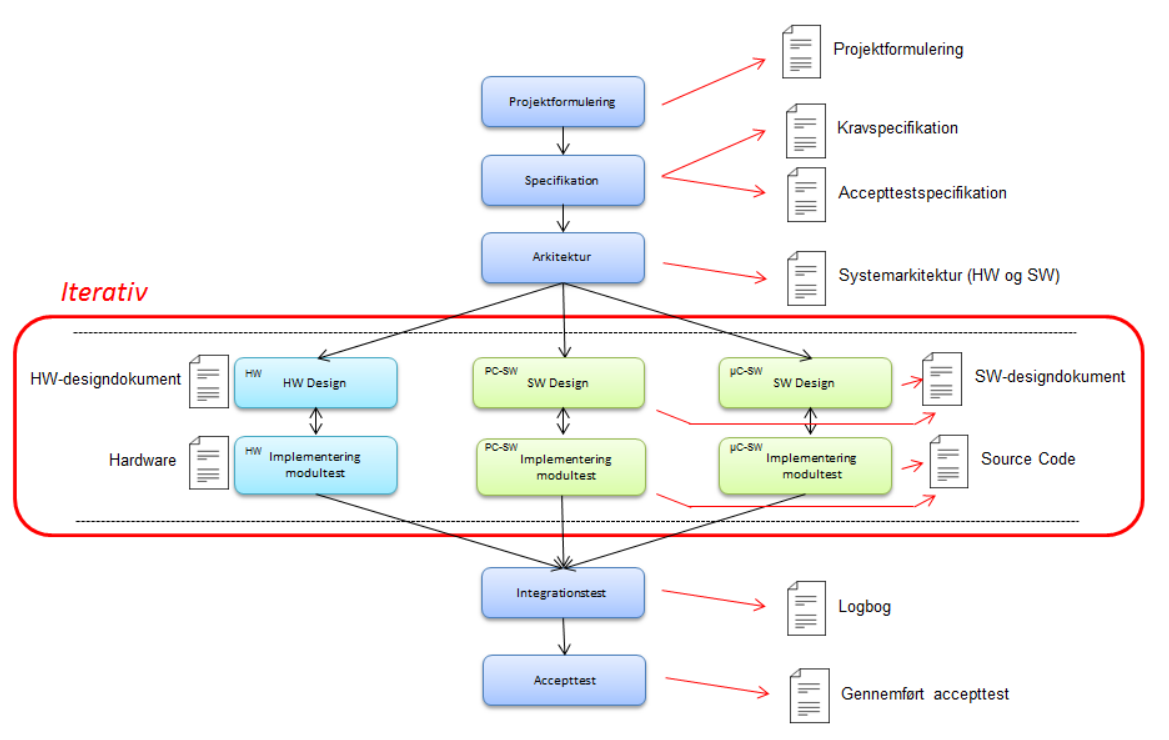
\includegraphics[width=0.8\textwidth]{Figurer/AseModellen}
	\caption{ASE-modellen}
	\label{fig:ASE_model}
\end{figure}
For at forstå ASE-modellen er det vigtigt at gennemgå Use Cases; et værktøj, som skal beskrive interaktioner mellem diverse aktører og selve systemet. Sammen med de ikke-funktionelle krav opnås et overblik over hvilke funktionalitetskrav, der stilles til systemet. På baggrund af kravspecifikationen kan accepttesten efterfølgende udarbejdes. I dette projekt er hardware- og software design implementering på lige fod, da projektet består af begge ting ligeligt.\\
\newline
V-modellen \cite{V-model} er en faseopdelt udviklingsmodel, der også er værd at nævne i dette projekt. Den beskriver udviklingsfaserne og testfaserne sideløbende i forhold til projektet, og den er derfor benyttet til dette projekt sideløbende med ASE-modellen. Modellen fungerer således, at specifikationen af test foregår parallelt med udviklingen af selve systemet.
\begin{figure}[H]
	\centering
	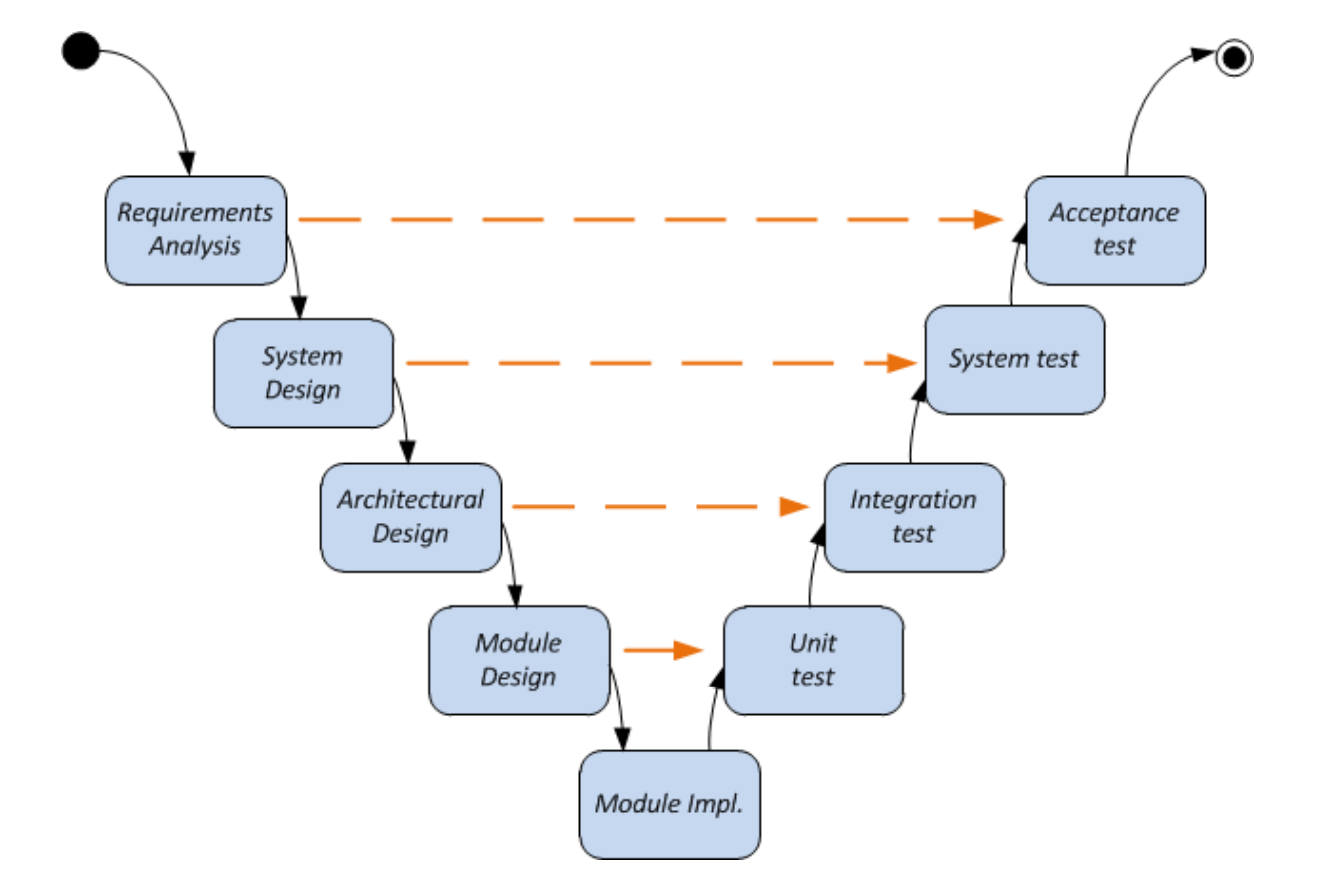
\includegraphics[width=0.6\textwidth]{Figurer/VModellen}
	\caption{V-model}
	\label{fig:V_Modellen}
\end{figure}
Den er blevet benyttet til hardware og software udviklingen. Hardware og software skulle begge teste deres funktioner inden nye faser blev igangsat, for at verificere om disse funktioner virkede korrekt gennem forløbet. Fordelen ved at teste på forskellige niveauer er, at det skal sikre de udviklede delsystemer, således at de virker som planlagt. Det er vigtigt, at hver fase er udført, før den næste fase påbegyndes. 
\newline

Vandfaldsmodellen \cite{Vandfalds-model} er også blevet benyttet under dette projekt. Softwareudviklingen bærer præg af vandfaldsmodellen, da udviklingen er opdelt i faser, hvor hver fase er blevet gennemført, før den næste er påbegyndt. Dette er i relation til V-modellen, som blev beskrevet før og den er, som vist på figur XX, konstant strømmende nedad. 

\begin{figure}[H]
	\centering
	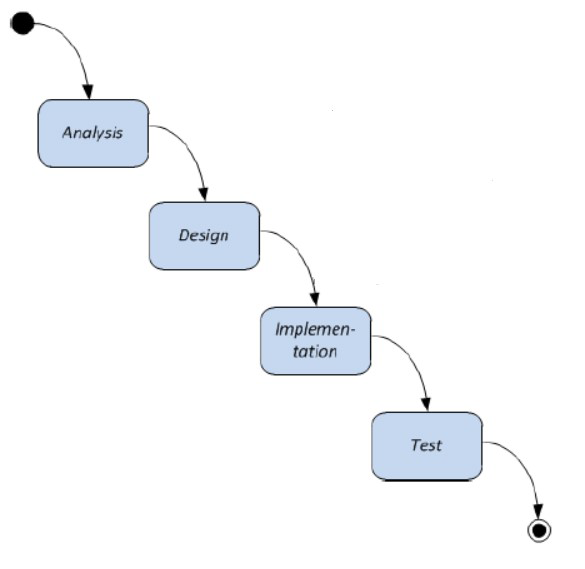
\includegraphics[width=0.4\textwidth]{Figurer/VandfaldsModellen}
	\caption{Vandfalds modellen}
	\label{fig:vandfalds_model}
\end{figure}


\section{Projektstyring}
Projektet er udarbejdet over et helt semester, hvor undervisningen og forelæsningerne delvist har udgjort grundlaget for teorien benyttet i dette projekt. Der blev i starten udarbejdet en tidsplan, som dog var mulig at ændre undervejs, men med faste deadlines, der skulle overholdes. Hovedpunkterne kan ses i denne tidsplan, som er vedlagt i bilag XX. \\
Projektgruppen har bestået af 6 gruppemedlemmer, som er blevet delt i 2 fokusområder, hardware og software.Fordelingen blev udarbejdet efter den enkeltes ønske. Gruppen har derfor været afhængig af at der var god kommunikation mellem de to undergrupper, derfor har hver arbejdsgang været i samarbejde. Da gruppen har været opdelt, har der været projektmøde hver uge, hvor gruppen har opdateret hinanden og vejleder. \\
Under projektet har alle medlemmer været med til, at sikre en administrativ kæde af deadlines til individuelle opgaver, samt dagsordener til hvert møde. Disse deadlines har sikret at opgaverne er blevet opfyldt op til møderne, for at hindre langsomme arbejdsprocesser. Da der har været overlap mellem de forskellige opgaver er arbejdet foregået flydende for at sikre, at der blev testet. 

\section{Metoder}
Til at kunne overskue arkitektur og designet af projektet, er flere forskellige arbejdsmetoder benyttet for at skabe det bedst mulige resultat. 
For at finde, hvad blodtryksmåleren skal gøre, er der blevet udarbejdet Use Cases. Disse beskriver systemet funktionalitet. Use Cases viser, hvad brugeren skal opleve fra systemet, men ikke, hvordan det sker. I Use Case diagrammet bliver det også vist, hvilke aktører der findes og hvordan de interagerer med systemet.   \\
I projektet bruges accepttest til at teste blodtryksmåleren. Dette gøres ud fra kravspecifikationerne, hvor det er angivet, hvilke krav der er til systemet. \\Accepttesten er en test, hvor der beskrives, hvad der skal ske og, hvad brugeren skal gøre. Testen er for at undersøge om produktet opfylder de krav, som der er blevet sat for det. Accepttesten giver et godt overblik for udvikleren og for kunden, der nemt og hurtigt kan se om produktet virker som det skal. \\
\newline
Til  beskrivelse af design af software og hardware er diagrammer og skemaer blevet udarbejdet i SysML og UML. SysML er et grafisk modelleringssprog, som kan bruges til at overskueliggøre systemer. \\
Til software er der blandt andet lavet en applikationsmodel i SysML, som består af et domæne-, klasse- og sekvensdiagram. \\
Domænemodellen viser sammenhængen mellem blokkene i systemet. Blokkene findes i Use Casene og derved bliver disse to ting koblet sammen. \\
Klassedigrammet viser, hvilke metoder blokkene har og hvordan de kommunikerer med hinanden. Her findes domæne-, kontrol- og grænsefladeklasser. Kontrolklasserne beskriver, hvordan data behandles mellem domæne- og grænsefladeklasser. Domæneklasser indeholder funktionalitet fra den pågældende softwareblok. Grænsefladeklasserne viser, hvordan, systemet interagerer med omverdenen. Diagrammet gør det nemmere at fremme en lav kobling og høj samhørighed i softwaren.\\
Sekvensdiagrammet fortæller, hvad der sker i selve koden. Igen går det ud fra Use Casene, hvor vægten nu er på softwaredelen. Derved beskrives det, hvordan metoder bliver kaldt og hvordan de forskellige klasser interagerer. Hver Use Case skal her gennemgås i software, så der skabes et overblik over vejen gennem koden.\\
\newline 
For at skabe et overblik og indsigt i koden, er der i UML udarbejdet et aktivitetsdiagram og et klassediagram. Aktivitetsdiagrammet går i dybden med en specifik metode. Det er kun blevet gjort for relevante metoder. Her tydeliggøres det, hvordan hver metode fungere og, hvad den indeholder.  Klassediagrammet fortæller hvilke metoder, en klasse indeholder og hvordan klasserne hænger sammen.\\
\newline  
Til hardwaren er der blevet brugt Block Definition Diagram(BDD), som viser hvilke blokke et system indeholder og hvilke porte de har. BDD er lavet til at give et overblik over systemet. Ud fra BDD’et er et Internal Block Diagram(IDB) blevet lavet. Her vises, hvilke signaler som findes i systemet og hvordan de sendes rundt. Her vises portene igen og der skal være overensstemmelse  mellem BDD og IBD.    

\section{Systemarkitektur}
\subsection{Hardware}
\subsection{Software}

\section{Problemidentifikation (design)}
\subsection{Hardware}
\subsection{Software}

\section{Implementering}
\section{GUI-beskrivelse}
\subsection{Algoritmer (grænseværdier)}
\subsection{Filteret/Ufiltreret}
\subsection{Lagring af data i Database}

\section{Test}
\section{Resultater og diskussion}
\section{Udviklingsværktøjer}
Gennem projektarbejdet har vi anvendt en række forskellige værktøjer til udvikling af blodtryksmåler-systemet. Disse er yderligere uddybet herunder.

\textbf{Visual Studio 2013}

Softwaredelen af projektets programmering er skrevet i sproget C-sharp. Her er Visual Studio 2013 anvendt som kompiler, da programmet gør det nemt at omskrive tekst til kode. Visual Studio 2013 indeholder også funktionen Windows Form Application, der visuelt kan fremstille de ønskede resultater i form af knapper, grafer og labels mv. i en samlet brugergrænseflade, som aktøren interagerer med. 

\textbf{Microsoft Visio 2016}

Microsoft Visio er et tegne værktøj, der i dette projekt er anvendt til at designe både SysML og UML diagrammer, som benyttes ved organisering af hardware og software design. Microsoft Visio er det oplagte valg, da diagrammer lavet i programmet får et enkelt og overskueligt udseende, og dermed fremstår det tydeligt for læseren hvad diagrammet vil vise.

\textbf{Analog Discovery og Waveform fra Digilent}

Analog Discovery og Waveform er i projektet benyttet som omformer og signal generator under testfasen. Her fungerer Analog Discovery som en Waveform generator, så et analog signal kan sendes videre ind i lavpasfiltret, forstærkeren og derefter ind i DAQ’en. I den endelig implementering erstattes Analog Discovery og Waveform med transduceren. 

\textbf{NI-DAQmx}

NI-DAQmx er et værktøj udarbejdet af National Instruments, som anvendes til at omforme det indkomne analoge signal fra transduceren (Analog Discovery) til et digital signal. Værdier fra NI-DAQmx er af en type som kan anvendes i selve softwarekoden. 

\textbf{LaTeX}

LaTeX er anvendt i projektet til design og opsætning af projektrapport og projektdokumentation. LaTeX er god til tekstformatering, hvor opsætning og strukturer defineres samlet for hele rapport, samt god til versionsstyring. Til at skrive selve koden benyttes programmet TeX-maker som kombiler. 

\section{Opnåede resultater}
\section{Perspektivering - Fremtidigt arbejde}
I fremtiden vil blodtryksmåleren kunne udvides gennem flere muligheder. Da blodtryksmåleren er lavet til forskningsbrug, er der ingen idé i at udvide mod patienter.  En forlængelse af systemet kunne derimod være en metode, som skal kunne vise gemte målinger. \newline Et log-in vindue er en anden ting, som kunne forbedre systemet, for på den måde at skabe større sikkerhed for forskeren og dataen. Et log-in vindue vil gøre at, en forsker kan være sikker på at hans målinger og forskning ikke kan tilgås af andre. Det kræver en større udvidelse, hvor der skal laves et log-in vindue og en database, hvor password og brugernavn gemmes. Der skal også laves en metode, som kan tjekke om det indtastede password og brugernavn passer over ens med det i databasen. 
\newline
Generelt skal de standarter, som findes for blodtryksmålere undersøges grundigere. Specielt brugergrænsefladen, men også resten af systemet som enheder og visning af graf, skal rettes til efter de passende standarter.
\newline 
Hvis systemet ydeligere skulle tilpasses forskning, kunne det gøres gennem en bedre navngivning af data i tabellen eller et bedre overblik over, hvordan data bliver gemt f.eks. gennem en liste for de gemte målinger. På den måde vil det blive nemmere for forskeren at finde frem til gamle målinger.   
\newline 
I forhold til hardware er målet, at det hele skal samles i en kasse. Så det på den måde ikke er muligt at ændre eller stille ved det. Derved skal filteret og forstærkningen laves på en printplade. Samtidigt skal det ved kassen være en plads til batterierne, hvor det er muligt at kunne skifte dem, når nødvendigt. Derved fås en kasse, som nemt kan flyttes rundt på og som ikke er i fare for at gå i stykker.   